\section{寮内議論で遊ぼう！}
\rightline{（文責：アメリカムシクイ）}
\subsection{1.はじめに}
熊野寮の意思決定は議論でなされる。「徹底討論の原則\footnote{「当事者間解決の原則」、「公平平等の原則」に並ぶ、寮の三大原則の一つ。人によって解釈が分かれる。ただ、様々な論考を読む限りでは、「外的状況と組織の状態の二つを把握するために、意見を出し合いながら各自の持っている情報を共有するプロセス」と捉えていることが多い。}」という標語にも見られるとおり、安易な多数決に頼ることなく全会一致を目指して議論を尽くすという方法は、意思決定のための基本的な理念である。
\par
寮の議論に参加していると、議論には底知れぬ奥深さがあるということをいつも実感させられる。意見からその人の根底にある問題意識を見抜くにはどうすればよいか。拾ってきた問題意識を解消するためには、どのように提起を変更すればよいのか。そういったことは、いくら大学の勉強に励んでもわからない。議論という複雑系と腰を据えて向き合ってみて初めて体得できる類のものであるように思われるのである。「寮内議論で遊ぼう」というタイトルが意味するように、本記事は議論というツールと向き合い、遊んでみることでその深淵を覗き込もう、という試みなのだ。
\par
議場で意見を述べるときは、現状に至るまでの議論の流れを踏まえておかなければならない。そのためにはこれまでに出てきた意見を理解し、論点を把握する必要がある。意見は「発言内容」と「他の意見との関係性」という二種類の情報を持っているので、意見を理解することは、相手の視点に立って内容を理解することと、意見の向き先や属性を把握することの、二つの営みに分かれる。本記事で考えたいのは後者である。
\par
議論は意見の交換を繰り返すことで進行する。これは議論が普遍的に持つ性質であり、ひとつひとつの議論は意見交換という骨格に、具体的な内容を肉付けしたものとして捉えることができる。それゆえ、逆に具体的な議論から意見の内容を捨象すれば、意見交換の枠組みだけを取り出すことができる。意見どうしの関係性を把握するということは、議論の骨格を捉えるということに他ならない。
\par
そこで本記事では、意見交換の樹構造に注目し、議論の骨格を図によって表現することを試みる。以下、議論の骨格を表現した図のことを「議論樹」と呼ぼう。まずは議論樹の記法を導入し、具体的な議論に対して議論樹を描く。この際、具体例に少し手を加えることで、議題や出てくる意見が同じ議論でも、異なる議論樹を得ることができる。最後に議論樹の応用として、複数の議論樹を比較して分かることを述べる。
\par
これまでにも議論の理念的な考察や、意見者の分類など、議論を題材にした論考は既に存在する\footnote{過去の入寮パンフレットの記事としては、「熊野自治三論（2022）」、「寮議論で現れがちな論者KUMANaverまとめ（2019）」など}。しかし、寮内議論を議論というツールそのものに焦点を当てて考察する試みは、筆者は見たことがない。本記事のように図などを用いて議論で遊ぶことで、寮の議論を少しでも面白いと感じてもらえれば幸いである。
\subsection{2.議論樹について}
\subsubsection{2.1.議論樹の記法}
\begin{figure*}
  \centering
  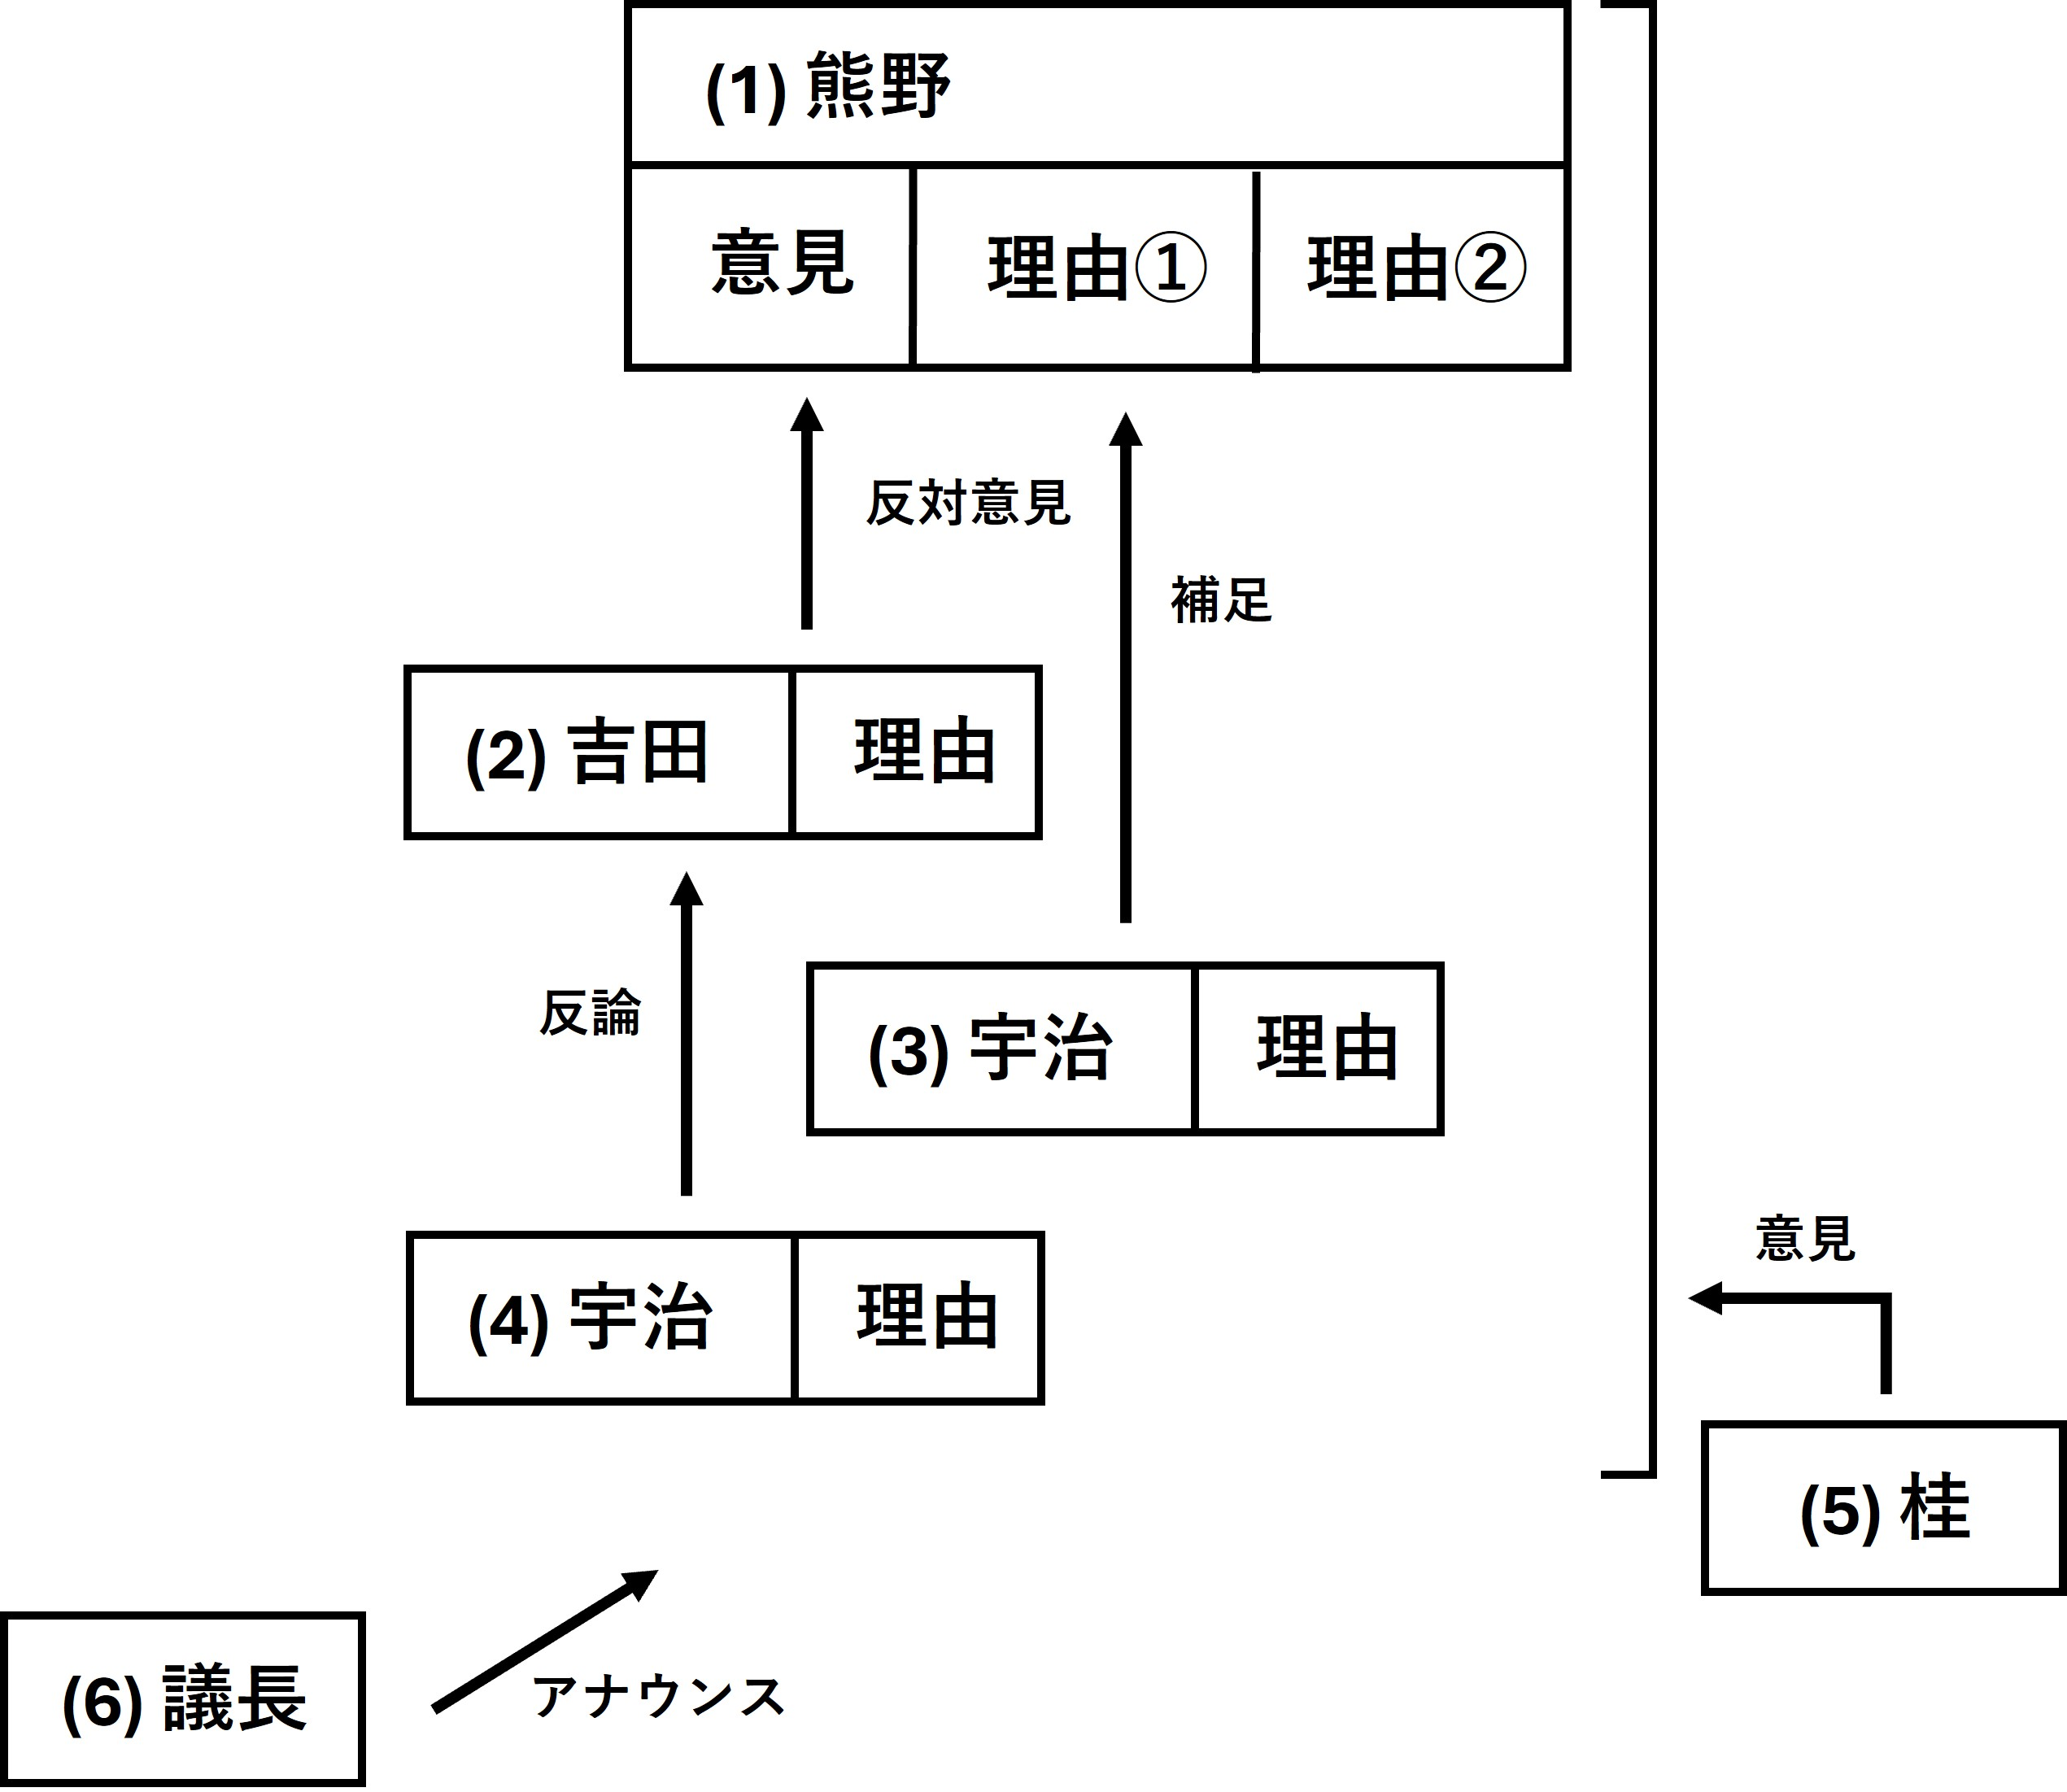
\includegraphics[height=8cm,width=9cm]{2026shinki/dormitory-discussion/figures/discussiontree_guideline.jpg}
  \caption{議論樹の一例}
  \label{fig:discussiontree_guideline}
\end{figure*}
議論樹とは、議論の構造を樹木のように図で表現したものである。図\ref{fig:discussiontree_guideline}は議論樹の一例だ。この議論樹がどのような議論を表現しているか考えてみよう。例えば、次のような議論が考えられる。
\par
まず、熊野さんが自身の意見を一つ述べる。本人の考えに加えて、主張を支える根拠を二つ挙げている。次に、吉田さんが熊野さんの意見に対して反対意見を表明し、その立場に立つ理由も付言している。続いて宇治さんが熊野さんの挙げていた理由の一つに対して補足意見と、その理由を述べている。再び宇治さんが、今度は吉田さんの反対意見に対して理由をつけて反論している。なお、宇治さんが表明した二つの意見は、一つの発言の中で連続して表明されたものかもしれないし、二つの発言に分けて述べられたものかもしれない。それから桂さんが熊野さんから始まり宇治さんまで続いていた議論に対して意見を表明し、最後に議長が議論を切って熊野さんが提示した論点に関する議論が終了する。
\par
こうしてみると、議論樹が（多少曖昧なところはあれど）上手く議論の構造を表現できていることが分かると思う。より厳密に議論樹の記法を述べると、以下のようになる。
\begin{enumerate}
  \item 議論の発言をひとつひとつ分解し、その中の意見\footnote{ここで言う「意見」とは、発言者の立場や何らかの事実を述べたもののことである。立場表明は例えば賛成の立場や反対の立場が考えられる。より広く、「私は～と思います」という構文で主張されるもののことだ。一方で事実は、補足説明などを表す。「～の件については～です」といった構文で主張されるもののことである。}を述べられた順番に並べ、番号付けをする。
    \item 長方形の枠の中に意見の整列番号と、その意見を述べた参加者の名前を書き、一つの意見を表すブロックとする。もし意見に対して根拠が述べられていれば、それも合わせて長方形の枠の中に書く（図\ref{fig:discussiontree_guideline}を参照）。なお、発言者が意見を述べていることは明らかなので、省略することもある\footnote{図\ref{fig:discussiontree_guideline}では、熊野さんのブロックには意見を述べたことが記載されているのに対し、桂さんのブロックには意見を述べたことが記載されていない。しかし、桂さんが自身の意見を述べたことは矢印に書かれている文言からも明らかである。}。
  \item ブロックは、同一の論点に対する意見が縦一列に並び、異なる論点に関する意見が別の列に並ぶように配置する。新規論点のブロックは一番右の列におく。
  \item それぞれの意見に対し、その意見が向けられた先のブロックに向けて矢印を書く（図\ref{fig:discussiontree_guideline}では、吉田さんのブロックから熊野さんのブロックへ矢印が伸びている）。ただし、発言や意見が議場全体に向けられたものであった場合は、矢印を余白に向かって伸ばす。
  \item 4.で伸ばした矢印のそばに、意見の属性\footnote{例えば賛成意見、反対意見、補足、質問、返答などがある。賛成の立場も反対の立場も表明していない意見をたんに「意見」とラベリングしたりする。反対意見と反論の違いは、相手の発言内容を否定しているか否かで決まる。本記事では、反対の立場を表明しているだけなら反対意見、相手の意見や論拠に対して論陣を張って否定しているなら反論に分類した。}を書く。
  \item 特定の意見に対する意見ではなく、途中の議論に対して意見を表明している場合は、大きな括弧で意見の対象としている議論を囲い、上の記法と同様に図に記す（図\ref{fig:discussiontree_guideline}の桂さんの意見）。つまり、途中の議論全体に対する意見は新規論点として扱う。
  \item 議長や寮生大会の運営者が議場に向かってアナウンスしている場合は、一番左の列にブロックを配置し、余白に向かって矢印を伸ばす。なお、アナウンスに対して議論が生じた場合は、新規論点として一番左の列にブロックを配置し、あとは上の記法と同様に図に記していく。
\end{enumerate}
\subsubsection*{2.2.議論の例}
2.1.では議論樹の記法について述べた。この項では、具体的な議論に対して議論樹を作成してみる。以下に議論例を２つ挙げる。どちらも議題や意見は同じもので、扱う順番のみを変えた。できる限り寮の実際の議論を想像できるようなものを用意しているが、実在する人物や団体とは全く関係なく、貶める意図なども全くないことを注意しておく。
\par
舞台は寮生大会の自由討論\footnote{寮生大会のパートの１つ。寮生大会は形式的で色々と融通の利かないところがあるが、いざというときに臨機応変に対応できるようにするためのあそびの部分にもなっている。全寮生が一堂に会する唯一の機会なので、ここぞとばかりに寮生全員で話し合うための議題が持ち込まれたりもする。ただし、寮生大会で議論できる時間は多くて10時間程度しかないため、自由討論で何かが決まると思ってはいけない。}、議題は「朝寮食をご飯食にしましょう！【議論】【採決】」である。どうやらパンを提供する従来の朝寮食の形態から、お米を提供する形態に変更する提起がなされたようである。

\begin{description}
  \item[議論例１]\mbox{}\\
  \begin{description}
\item[提起者熊野：]朝寮食を現在のパン食からお米に変えたいと思います。理由は２点。ご飯の方がおなかにたまるから。そして、毎日菓子パンを食べるのは健康に悪いからです。お米にすることで、寮生の食生活を健康に保ち、勉学にも寮自治にも闘争にも思いっきり打ち込める寮にできると考えています。
\item[祇園：]提起者へ質問です。お米というのは具体的に何ですか？雑穀米ですか？
\par
\centerline{（ガヤ：しょうもな。）}
\item[熊野：]白米を想定しています。
\item[北白川：]お米を提供するとなると、朝早起きして炊くか、前日に炊いて保存しなければなりません。前者は厨房員がやるのか炊事当番の人がやるのか分かりませんが、いずれにせよ負担が大きいと思います。後者については衛生面から問題があると考えます。この点について、提起者はどのようにお考えでしょうか？
\item[熊野：]炊事当番の人が炊くのを考えてました。負担が大きいという指摘は持ち帰って検討します。
\item[議長：]他に質問などある方いますか？
\item[山科：]私はご飯食への変更には断固反対です。たくさんある菓子パンの中から選ぶ楽しみがあるから毎日早起きできているんです。普段朝寮食を食べている方はいつも食べてるパンを想像してみてください。私はメロンの妖精とアーモンドカスター\footnote{いずれも実際に朝寮食で提供されているパンの名称。メロンの妖精はメロンパンにメロン味のするつるつるな生地がコーティングされ、中にメロンクリームが詰まったパンで、アーモンドカスターはデニッシュにアーモンドとカスタードをトッピングし、アイシングをしたパンである。筆者の一推しはさくさく三角ショコラやショコラホイップパイだ。オレンジデニッシュなども高級感があって好きである。}が大好きです。これらを食べられないのであれば、もう寮食を食べる意味なんてありませんっ！
\par
\centerline{（ガヤ：ナンセンス！！食堂防衛しろ！！）}
\item[議長：]恐らく今おっしゃったのは好みのパンが食べられなくなるから反対だという意見だと思うのですが、好き嫌いに立脚する意見まで扱い始めるとキリがないので、休憩時間中にでも提起者と個別に討論してほしいと思います。新規の意見がある方h...
\item[山科：]勝手に決めつけないでください！明らかにこれは全寮的な問題じゃないですか！朝寮食に楽しみを見出せなくなって朝起きられなくなったりしたら、１,２限に出席できなくなって留年する寮生や体を壊す寮生が増えるんですよ！
\par
\centerline{（議場騒然。議長団内で協議が始まる。）}
\item[議長：]分かりました。決めつけたのは謝ります。議場で意見がある人はいますか？この論点に関する意見でも新規論点でも構いません。
\item[祇園：]先ほどの私の質問に重ねて質問です。産地はどこでしょうか。夜寮食と異なりタイ米などであれば何らかの形で調理しないと美味しくないので朝寮食には向いていないと思うのですが。
\item[熊野：]あー、はいはい。国産の白米です。
\item[議長：]他に意見ある方はいますか？
\item[今出川：]提起者の問題意識には共感しますが、先ほどの北白川さんの指摘は的を射ていると思います。そこで、折衷案としてタコスにするのはいかがでしょうか？ピザトーストが提供されていることから野菜の保存はできるはずなので、野菜の量やバリエーションを増やし、夜寮食のドレッシング\footnote{夜寮食ではドレッシングをかけることができる。しかし、別にドレッシングなどかけなくても寮食は美味しい。}の要領でソースも用意し、パンの代わりにタコスを提供して野菜を摂取するというのはいかがでしょうか？
\par
\centerline{（ガヤ：それピザトースト\footnote{朝寮食では食パン（正式名称は「食パン」ではない）を選ぶこともできる。食パンを選ぶと野菜を一袋とることができ、それを使ってピザトーストを作るのがメジャーな食べ方の一つだ。}でよくね？）}
\item[議長：]これに対して提起者の方返答をお願いします。あ、烏丸さんがどうしても今質問したいことがあるそうなので先にそちらを扱います。
\item[烏丸：]先ほどの山科さんの意見に対してです。選ぶ楽しみが必要なのであれば、ふりかけを用意すればいいのではないでしょうか。
\par
\centerline{（ガヤ：さえぎってまでそれ聞くか？）}
\item[伏見：]熊野寮生にふりかけなんて与えたらみんなご飯にドバドバかけてすぐなくなっちゃうから意味ないと思います。しかもふりかけが何で美味しいか皆さん分かりますか？たくさん食塩が入っているからです。そんなもん寮生に食べさせたら菓子パンよりも健康に悪いでしょうよ。皆さんもう少し考えて意見しませんか？
\par
\centerline{（議場紛糾。議長団内で協議が始まる。）}
\item[議長：]ええっと、次々に論点が出てきてこのままでは議論が収束しないので、この議題に関しては継続討論とします。最後に堀川さんがdiscord\footnote{熊野寮では公式の連絡ツールとしてdiscordを用いている。寮生大会の際にはdiscord上でも意見を集めたりする。}に書いた意見を共有したいそうなので、堀川さんの発言で議論を終了します。
\item[堀川：]先ほど折衷案の提示がありましたが、ここまでの議論で提起者の問題意識への反対意見が出ていないことを考えると、北白川さんがおっしゃったような課題さえ解決できれば、ご飯食にするのが寮自治会として取るべき選択であることは一致が取れると思います。これは学生の福利厚生の問題なので、本来は大学当局がご飯を炊くための厨房員を雇うべきものであるはずです\footnote{やや暴論に見えるかもしれないが、厨房員の給料を支出しないという攻撃は度々起こっている。そのような場合は大学の代わりに寮の予算から支出する。堀川が言っているのは、「ご飯食にした方が学生が勉強その他活動に打ち込める。寮は大学の福利厚生施設なので、当然大学は学生の活動を後押しするべきである。そのため、ご飯食にするために新たに厨房員を雇う必要が出てきたならば、大学が厨房員を雇うべきだ。ついでにこれまで厨房員の補充などをサボタージュしてきたことも追及したい。」ということである。}。そこで、提起者の問題意識などを整理して再来週の窓口交渉\footnote{寮生で集まって厚生課窓口に交渉しに行くイベント。両者の間で今後の対応が決まることもあるが、向こうが官僚答弁に終始し、話が全く進まないこともある（この傾向は処分など、学内政治に関わる話題に顕著に見られる）。}に持っていき、ご飯食に変えるよう当局に働きかけるべきだと考えます！ご飯食を実現するためにも、寮生の皆さんは窓口交渉に結集しよう！
\item[議長：]ありがとうございます。それではこの議題に関しては継続討論とし、窓口交渉の議題にするかどうかなども含めて今後の会議で議論していくことにするのがよいと思います。自由討論の議論は終了します。
  \end{description}
\end{description}
上の議論例は、論点が錯綜していて分かりにくい。議長が論点ごとに交通整理したとすると、次のようになる。なお、必要に応じて議長からのアナウンスを変えている。
\begin{description}
  \item[議論例２]\mbox{}\\
  \begin{description}
\item[提起者熊野：]朝寮食を現在のパン食からお米に変えたいと思います。理由は２点。ご飯の方がおなかにたまるから。そして、毎日菓子パンを食べるのは健康に悪いからです。お米にすることで、寮生の食生活を健康に保ち、勉学にも寮自治にも闘争にも思いっきり打ち込める寮にできると考えています。
\item[祇園：]提起者へ質問です。お米というのは具体的に何ですか？雑穀米ですか？
\item[熊野：]白米を想定しています。
\item[祇園：]先ほどの私の質問に重ねて質問です。産地はどこでしょうか。夜寮食と異なりタイ米などであれば何らかの形で調理しないと美味しくないので朝寮食には向いていないと思うのですが。
\item[熊野：]あー、はいはい。国産の白米です。
\item[北白川：]お米を提供するとなると、朝早起きして炊くか、前日に炊いて保存しなければなりません。前者は厨房員がやるのか炊事当番の人がやるのか分かりませんが、いずれにせよ負担が大きいと思います。後者については衛生面から問題があると考えます。この点について、提起者はどのようにお考えでしょうか？
\item[熊野：]炊事当番の人が炊くのを考えてました。負担が大きいという指摘は持ち帰って検討します。
\item[今出川：]提起者の問題意識には共感しますが、先ほどの北白川さんの指摘は的を射ていると思います。そこで、折衷案としてタコスにするのはいかがでしょうか？ピザトーストが提供されていることから野菜の保存はできるはずなので、野菜の量やバリエーションを増やし、夜寮食のドレッシングの要領でソースも用意し、パンの代わりにタコスを提供して野菜を摂取するというのはいかがでしょうか？
\item[議長：]折衷案の提示がありました。これについて意見ある方はいますか？
\item[堀川：]折衷案の提示がありましたが、ここまでの議論で提起者の問題意識への反対意見が出ていないことを考えると、北白川さんがおっしゃったような課題さえ解決できれば、ご飯食にするのが寮自治会として取るべき選択であることは一致が取れると思います。これは学生の福利厚生の問題なので、本来は大学当局がご飯を炊くための厨房員を雇うべきものであるはずです。そこで、提起者の問題意識などを整理して再来週の窓口交渉に持っていき、ご飯食に変えるよう当局に働きかけるべきだと考えます！ご飯食を実現するためにも、寮生の皆さんは窓口交渉に結集しよう！
\item[議長：]ありがとうございます。他に意見ある方はいますか？
\item[山科：]私はご飯食への変更には断固反対です。たくさんある菓子パンの中から選ぶ楽しみがあるから毎日早起きできているんです。普段朝寮食を食べている方はいつも食べてるパンを想像してみてください。私はメロンの妖精とアーモンドカスターが大好きです。これらを食べられないのであれば、もう寮食を食べる意味なんてありませんっ！
\item[議長：]恐らく今おっしゃったのは好みのパンが食べられなくなるから反対だという意見だと思うのですが、好き嫌いに立脚する意見まで扱い始めるとキリがないので、休憩時間中にでも提起者と個別に討論してほしいと思います。新規の意見がある方h...
\item[山科：]勝手に決めつけないでください！明らかにこれは全寮的な問題じゃないですか！朝寮食に楽しみを見出せなくなって朝起きられなくなったりしたら、１,２限に出席できなくなって留年する寮生や体を壊す寮生が増えるんですよ！
\centerline{（議場騒然。議長団内で協議が始まる。）}
\item[議長：]分かりました。決めつけたのは謝ります。議場で意見がある人はいますか？この論点に関する意見でも新規論点でも構いません。
\item[烏丸：]選ぶ楽しみが必要なのであれば、ふりかけを用意すればいいのではないでしょうか。
\item[伏見：]熊野寮生にふりかけなんて与えたらみんなご飯にドバドバかけてすぐなくなっちゃうから意味ないと思います。しかもふりかけが何で美味しいか皆さん分かりますか？たくさん食塩が入っているからです。そんなもん寮生に食べさせたら菓子パンよりも健康に悪いでしょうよ。皆さんもう少し考えて意見しませんか？
\centerline{（議場紛糾。議長団内で協議が始まる。）}
\item[議長：]ええっと、次々に論点が出てきてこのままでは議論が収束しないので、この議題に関しては継続討論とします。窓口交渉の議題にするかどうかなども含めて今後の会議で議論していくことにするのがよいと思います。それでは自由討論の議論は終了します。
  \end{description}
\end{description}
これらを議論樹におこすと図\ref{fig:discussion_example_1}、図\ref{fig:discussion_example_2}のようになる。
\begin{figure*}
\begin{minipage}{0.49\columnwidth}
  \centering
  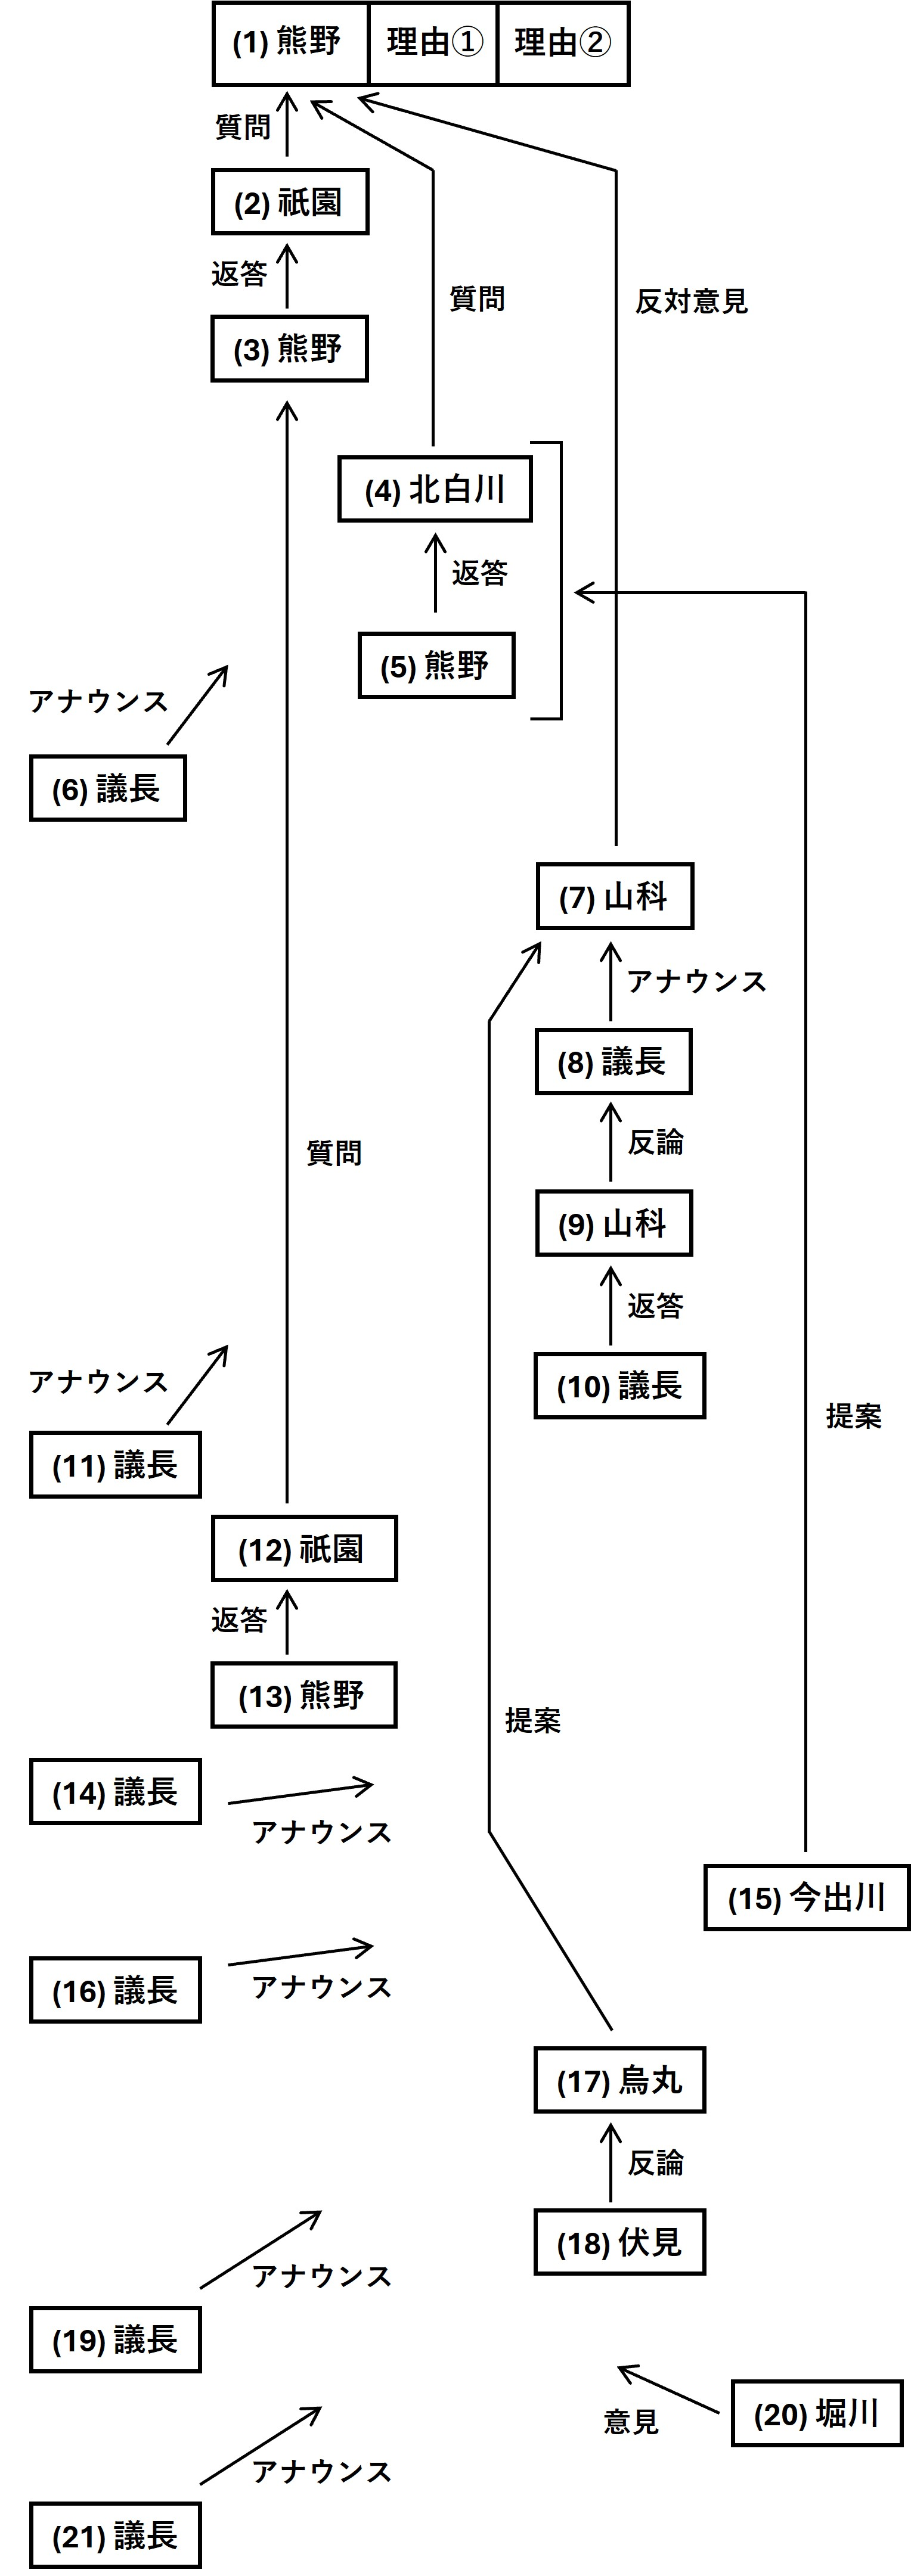
\includegraphics[height=20cm,width=7cm]{2026shinki/dormitory-discussion/figures/discussion_example_1.jpg}
  \caption{議論例１の議論樹}
  \label{fig:discussion_example_1}
\end{minipage}
\begin{minipage}{0.49\columnwidth}
  \centering
  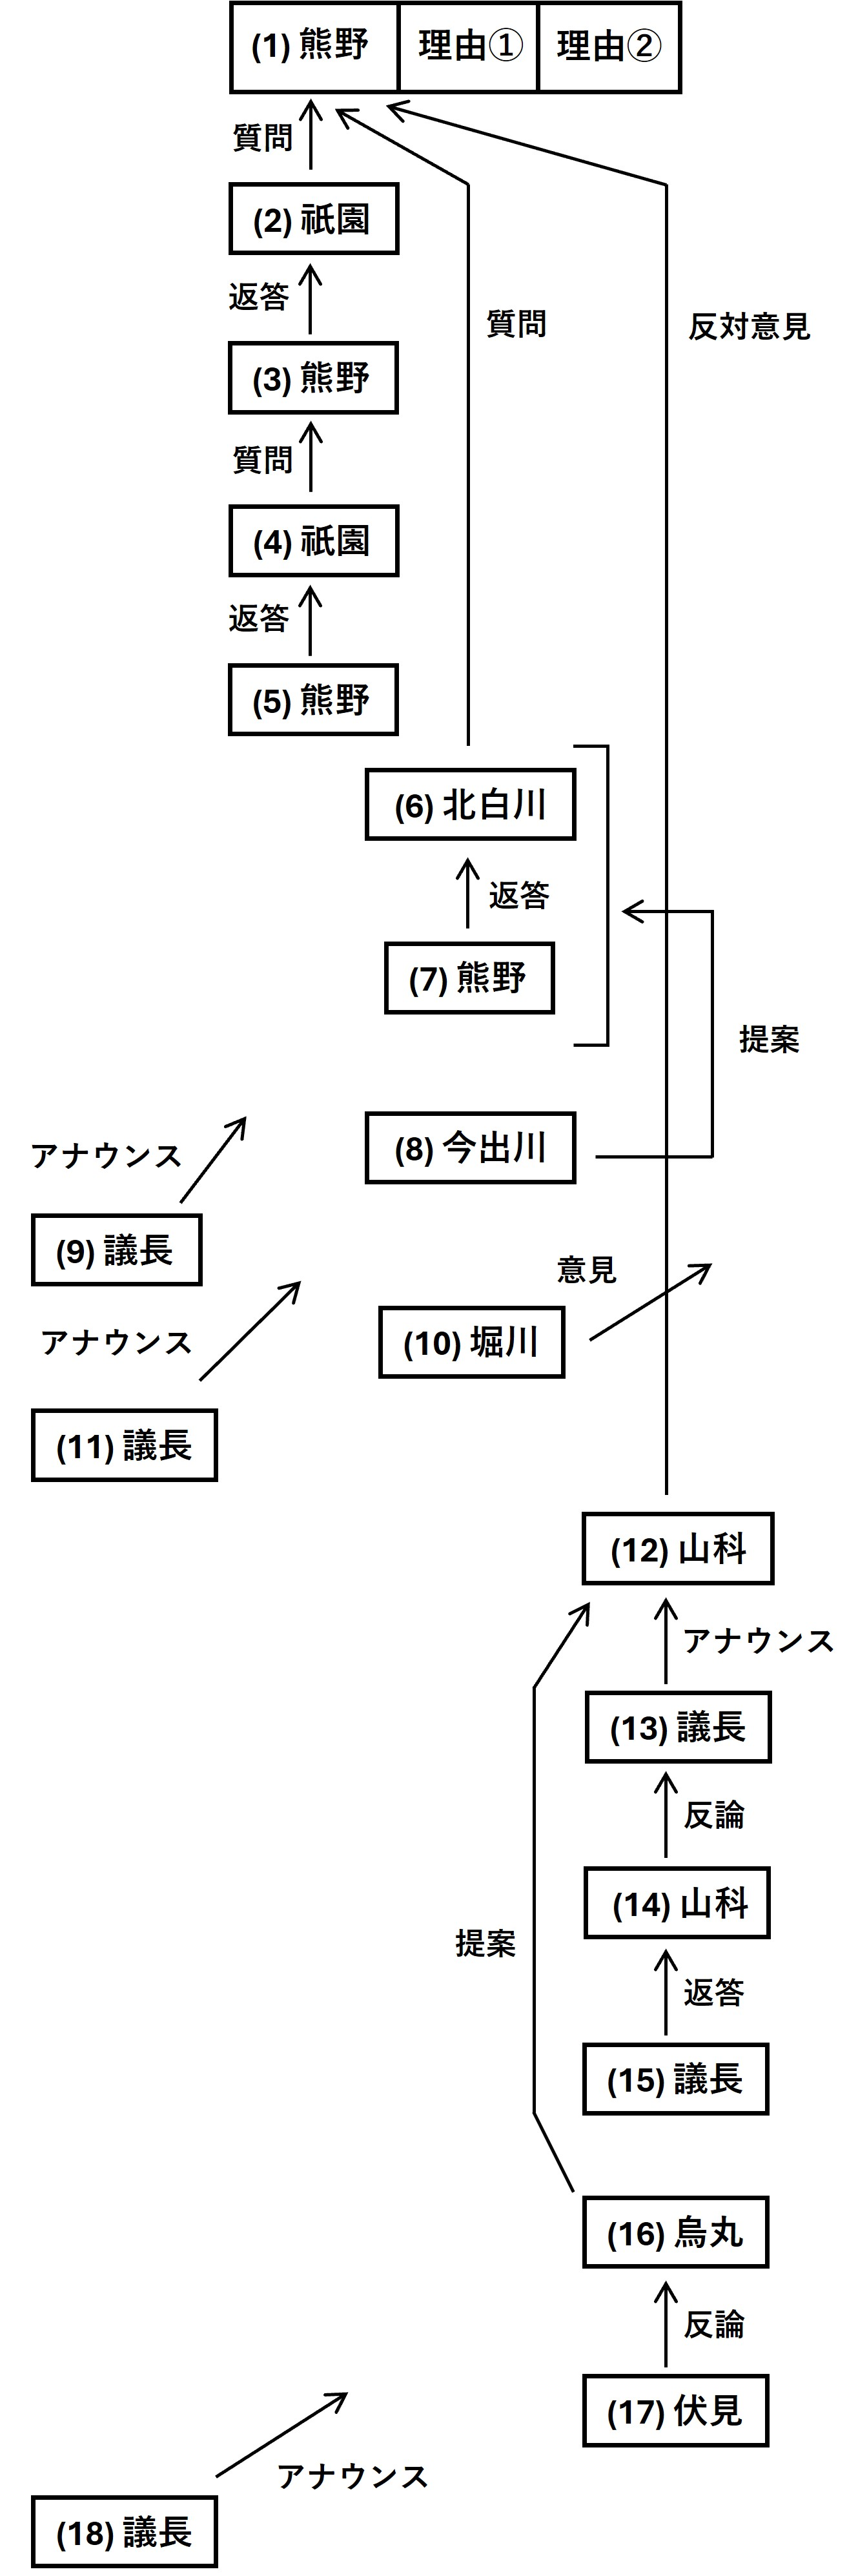
\includegraphics[height=20cm,width=7cm]{2026shinki/dormitory-discussion/figures/discussion_example_2.jpg}
  \caption{議論例２の議論樹}
  \label{fig:discussion_example_2}
\end{minipage}
\end{figure*}
\par
\subsubsection{2.3.議論樹の応用　～分かりやすい議論をつくるにはどうすればいいか～}
前項で議論の例を二つ紹介し、それぞれの議論樹を描いた。そこで、この項では議論樹の応用として、議論樹から議論についてどのようなことが読み取れるのか考えてみる。挙げた例は、いずれも論点や意見は同じで、扱う順番のみを変えた議論であった。これら２つの議論例、さらにはそれぞれに対応する議論樹（図\ref{fig:discussion_example_1}、図\ref{fig:discussion_example_2}）を比較した時、どちらが議論として分かりやすいだろうか。恐らく多くの人にとっては議論例２の方が分かりやすい議論であると思う。では、後者の議論の方が分かりやすいと感じるのはなぜだろうか。二つの議論例の違いはどこにあるのか。
\par
最も大きな違いは、論点ごとに議論をパッケージ化して扱っているかどうかである。例として挙げた議論では、熊野の提起に対して
\begin{itemize}
  \item 提供するお米の中身について（祇園の質問から派生）
  \item 現実的な課題の話（北白川の質問から派生）
  \item 選ぶ楽しみについての話（山科の反対意見から派生）
\end{itemize}
という三つの論点が生まれた。議論例１ではこれらの論点がごちゃ混ぜに扱われており、読み進めるうちに何の話をしているのかわからなくなってしまう。一方で議論例２では論点が一つずつ扱われているので、道に迷うことがない。この違いが、議論例１よりも議論例２の方が分かりやすいと感じる要因である。言い換えると、論点や発言の中身、意見の数などが同じ議論においては、論点を行き来する回数が少ない方が分かりやすいと感じるのではないか、と予想できる。
\par
これを踏まえると、参加者が付いてこれるように議事を進行するためには論点ごとに議論を尽くしていけばいいのではないか、という考えに至るのは自然なことだ。しかし、寮の議論はそう上手くはいかない。例に挙げた議論を現実の寮生大会でやろうとすると、祇園がお米の産地を尋ねる質問（議論例１の議論樹の(12)に相当）を思いつくのは、山科の一連の議論を聞いて「楽しみが必要ならカレーをかければいいのではないか」と思いついたことがきっかけであったり、今出川が折衷案（議論例１の議論樹の(15)に相当）をまとめるのに時間がかかり、先に山科の意見を先に扱ったりすることは往々にしてあることだ。また、仮に運よく論点ごとに議論を尽くしていけたとしても、論点が途中でいくつも分裂していってしまい、手に負えなくなることもある。
\par
このことから、議論の分かりやすさは他の要因によっても変わることが分かる。例えば、すぐに思いつくだけでも以下のような要因が挙げられる。
\begin{itemize}
  \item 議論の長さ
  \item 論点の多さ
  \item 論点を行き来する回数
\end{itemize}
\par
実際の議論では、上に挙げたような要素をその場でコントロールするのは困難であるため、より大雑把な方法で議論を整理することが多い。例えば、15分程度議論を中断して休憩する時間を設け、その間に意見がある人達を議長団席に集めて討論させる。そして休憩が終わった後に、論点整理した結果を議場に対して報告することで、議論の方向性を示す。そのように議論をパッケージ化して提示することで、議場の混乱を招くことなく議論を進めることができるのだ。確かに議長団席での議論が紛糾した際に休憩時間が必要以上に長くなってしまうという点や、頻繁に休憩をとることはできないという点がデメリットとして挙げられる。しかし、議場でとれる対応として最も有効なものであると筆者は考えている。他にも、寮生大会当日までにできる限り事前討論を尽くしておく、という対処法も一般的である。
\subsection{3.おわりに}
本記事では、議論を分析するツールとして議論樹を導入し、具体例を参照しながら議論樹の特徴や応用について述べた。議論樹を用いると、議論の構造を視覚化することができ、議論の複雑さを直観的に比較することができる。
\par
これまで見てきたように議論樹によって分かることがある一方で、意見を作るのにかかる時間や偶発的な思い付きは再現できないという欠点もある。議論樹のみから導くことができる結果が必ずしも現実において有益であるとは限らないという点は、本記事の試みが今後必ず解決せねばならない課題の一つであろう。また、議論樹をグラフ\footnote{頂点を辺で結んでできる図形のこと。数学ではグラフ理論という一つの分野を成しており、シンプルだが応用は広い。議論樹をグラフと見るには、発言のブロックを頂点、矢印を辺と考えればよい。}と捉えることで、議論という対象を数学的な言葉で理論化することもできる。この方面の考察も今後推し進める必要があるだろう。
\par
熊野寮を学術的に考察することは、筆者が入寮してから目標にしてきたことの一つであった。実際に議論を題材にした研究論文は数多く存在し、その切り口は理論的なものから実践的なものまで多岐にわたる。本記事で述べたことは、これらの膨大な蓄積の一つに過ぎない。その意味で、熊野寮という場所は学術の実践の場でもあり、興味深い対象でもあるのだ。